\chapter{Analýza a implementace serverové části}\label{ch:server}


Vzhledem ke změněým požadavkům a potřeby změny architektury bylo rozhodnuto přepsat celou implementaci serverové části od začátku.
Původní zdrojový kód bude sloužit pouze jako inspirace pro realizaci některých funkcionalit.


\section{Architektura}\label{sec:server-arch}

Při modelování poskytnuté domény do \g{MSA} je vhodné použít dekompozici úlohy na menší části s následujícím mapováním na služby.

Dekompozice se provedla na následující mikroslužby:



\begin{dl}
   \item[Users] – uživatelská data
   \item[Auth] – autentizační data, kontrola validity autorizačních údajů,
   \item[Projects] – služba pro správu projektovách dat.
   Ukládá v relační databázi metadata o projektech a deleguje úpravy obsahů na vnější Git úložiště
   \item[Interpreters] – správa registovaných interpretů
   \item[Communication] – zpracovávání komunikačních zpráv s uživateli
   \item[Localization] – správa překladů
   \item[Logger] – služba pro centrální ukládání a vyhledávání logů
   \item[Monitoring] – služba pro centrální kontrolování stavů mikroslužeb
\end{dl}

A pomocné organizační služby:

\begin{dl}
   \item[Router-orch] – služba řízení dotazů na mikroslužby ve vnitřní komunikaci,
   \item[Gateway] – služba řízení dotazů na mikroslužby z vnějšího prostředí,
\end{dl}

\begin{figure}[htbp]
   \centering
   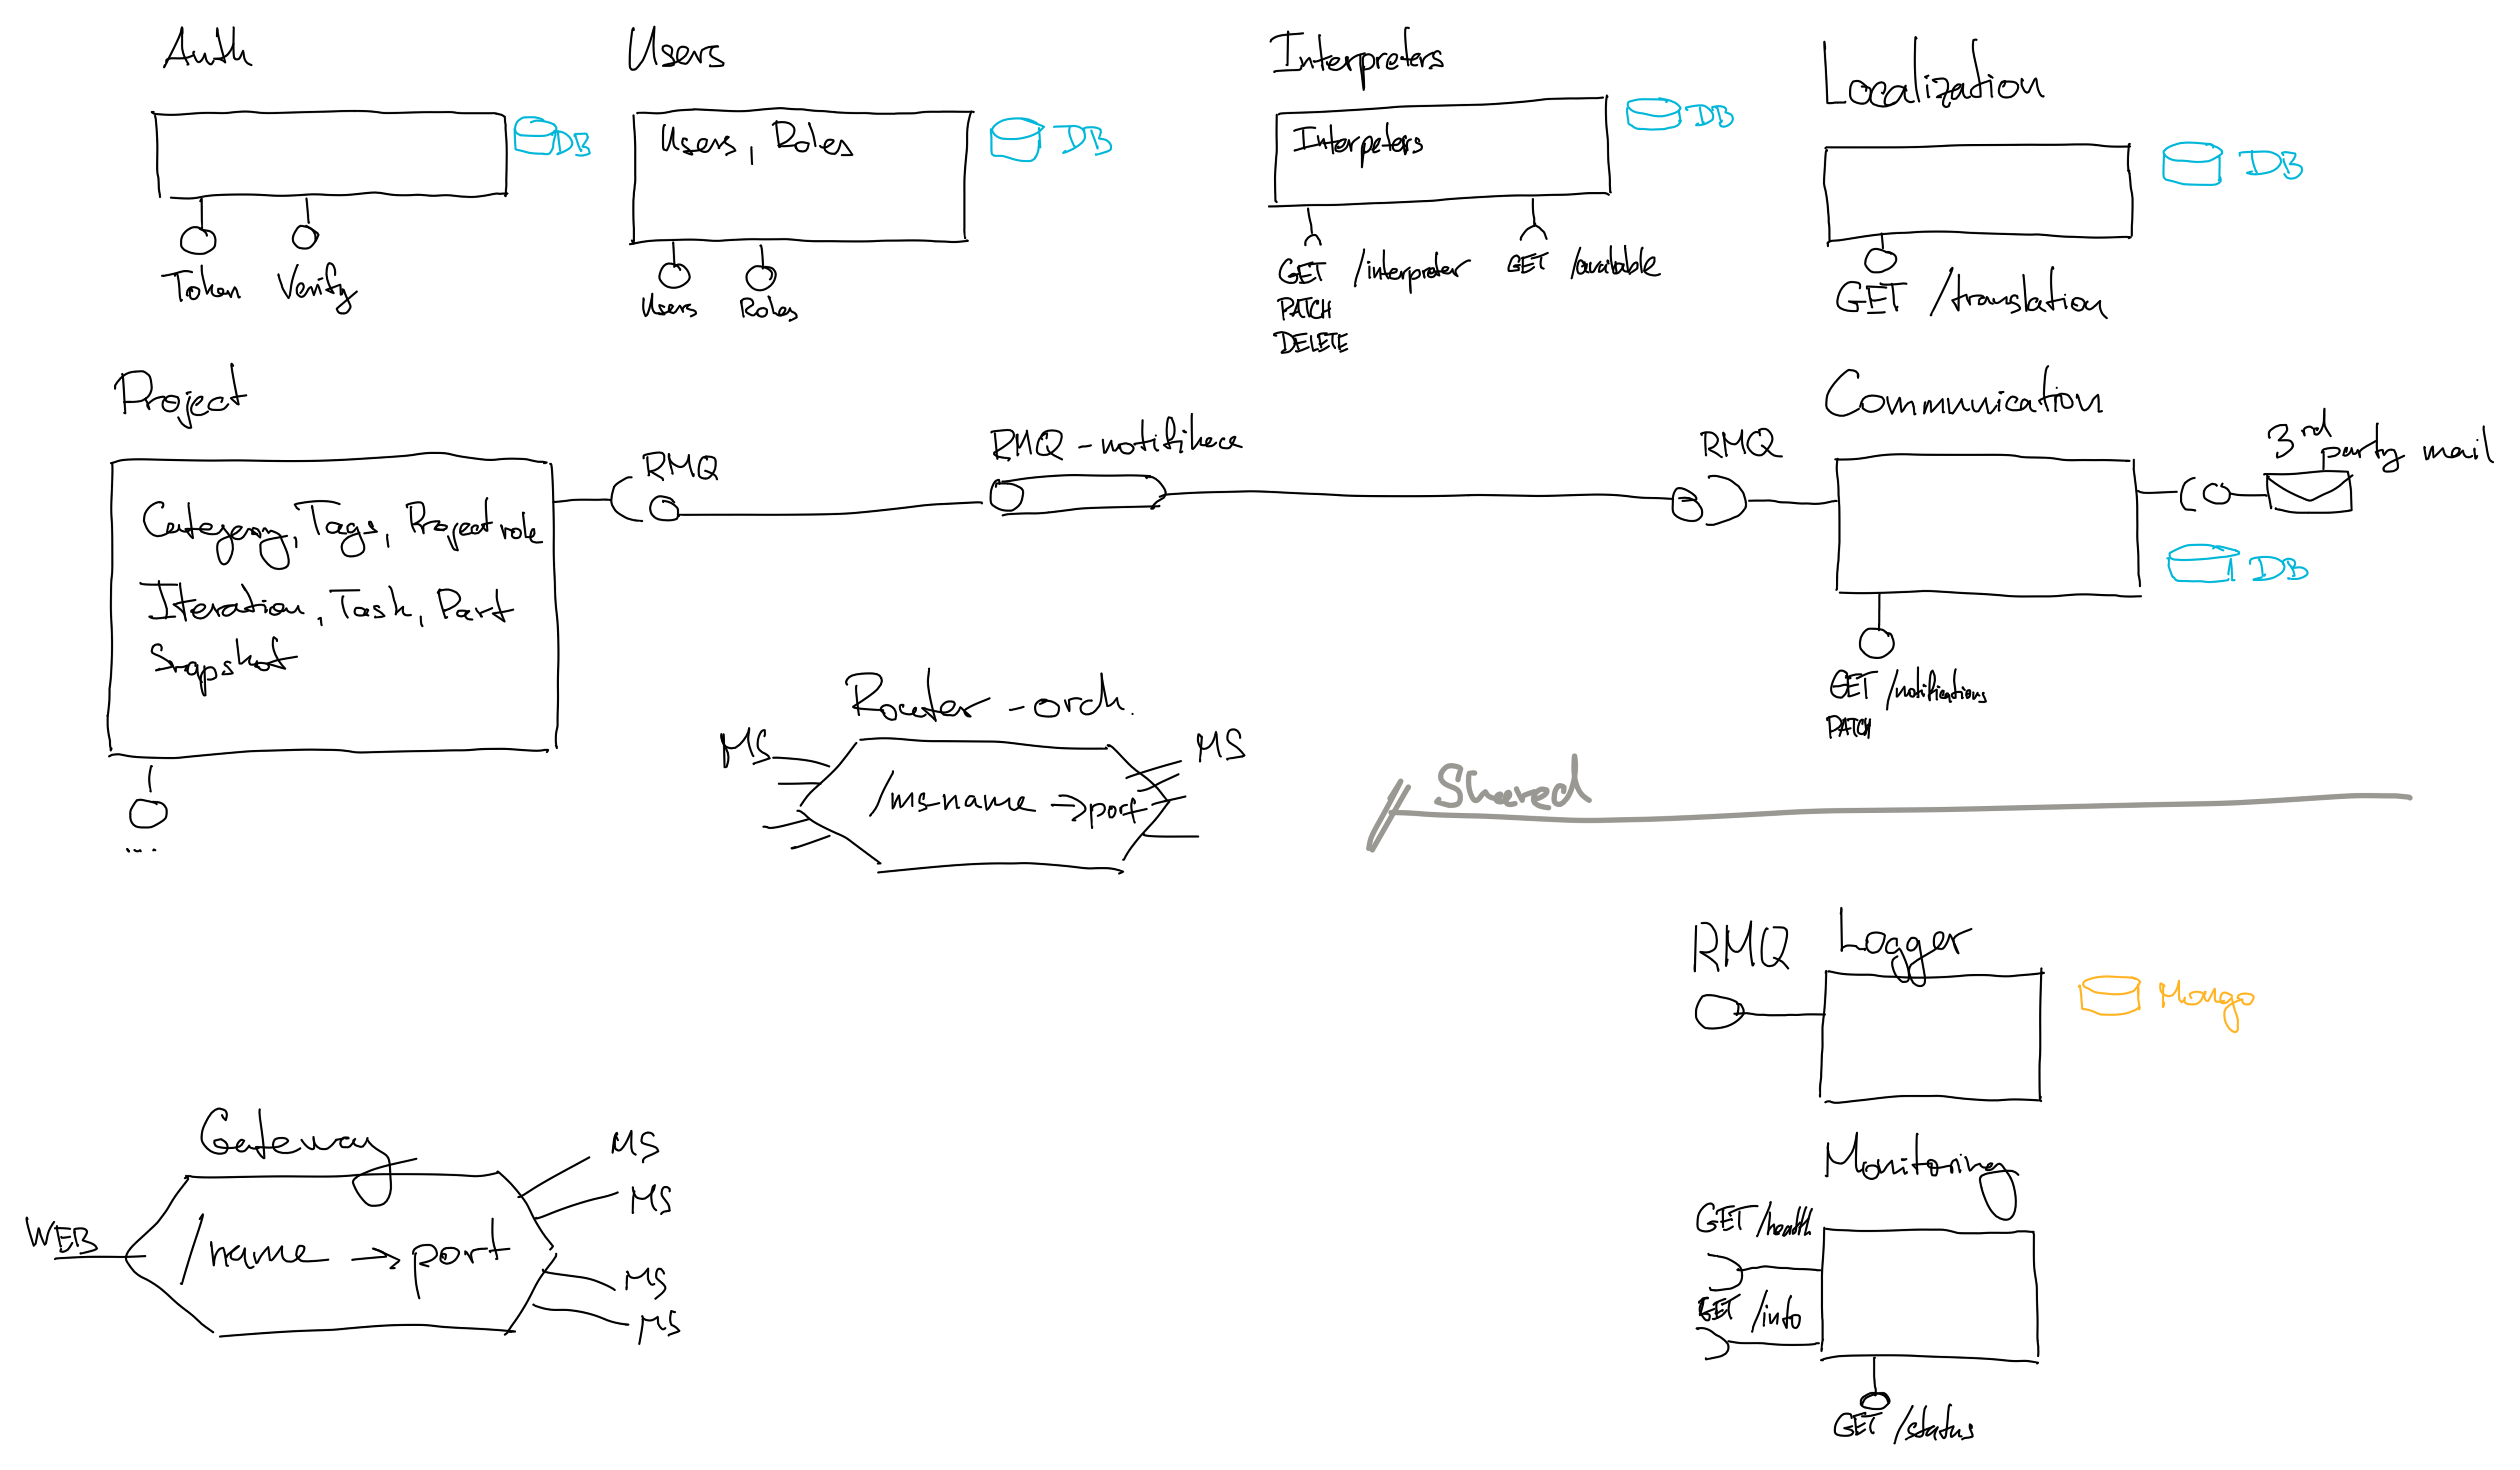
\includegraphics[max width=\textwidth]{assets/draft-server-arch}
   \caption{Architektura serveru}\label{fig:server-arch}
\end{figure}



\section{Šablona pro mikroslužbu}\label{sec:server-template}

Všechny mikroslužby v architektuře sdílí určité chování a poskytované rozhraní.
Vzhledem k požadavkům systému na základě předchozí analýzy byly vybrány následující návrhové vzory pro implementaci:
\TODO{seznam implementovanych vzorů}
Na obrázku~\ref{fig:ms-template} lze vidět vizuální znázornění rozhraní, které vzniklo jako následek výběru návrhových vzorů.


\begin{figure}[htbp]
   \centering
   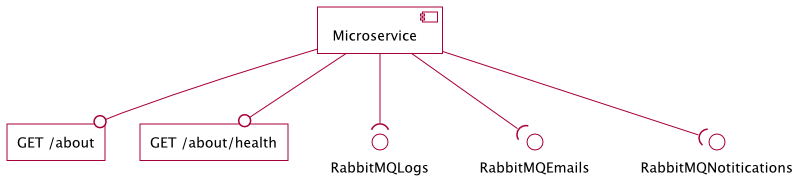
\includegraphics[max width=\textwidth]{assets/draft-ms-template}
   \caption{Standardizované rozhraní mikroslužeb}\label{fig:ms-template}
\end{figure}

Zarhnuje v sobě:

\begin{ul}
   \item \h{GET \g{REST} /info} pro získání základních metainformací o službě (například název, verze, vyžadované závislosti apod.),
   \item \h{GET \g{REST} /health} pro kontrolu, zda tato služba je dostupná,
   \item \h{RabbitMQ log} pro připojení se k RabbitMQ kvůli zápisu logů,
   \item \h{text log} pro běžnou kontrolu logů napřímo v \g{MS},
   \item jiné komunikační kanály pro poskytování svých možností.
\end{ul}



\section{Databáze a správa dat}\label{sec:server-db}

Pro správu dat v databázích byl vybrán vzor používající jednu databázi se sdíleným přístupem pro všechny \g{MS}.
Migrace



\section{Sestavování balíčku a kontejnerizace}\label{sec:server-compile}

Vzhledem k používaným technologiím zdrojový kód aplikací nelze spouštět bez předchozího zpracování.
TypeScript, jako samostatný jazyk, vyžaduje transpilaci kódu do JavaScript přes vhodný nástroj, například \h{tsc}.
Dle výchozího chování vytváří vedle každého rozpoznaného \h{.ts} souboru jeho transpilovanou kopii, importované a exportované části se neslučují.
V takovém stavu se \h{.js} soubory již dají spouštět za pomocí nástroje \h{node} (Node.js).

Obdobného chování, ale již bez explicitního transpilování, lze dosáhnout s pomocí nástroje \h{ts-node}.
Balíček \h{ts-node} je dle jednoho z autorů připraven pro produkční prostředí a program může být spuštěn bez dopadu na výkon~\cite{tsnodeprod}.
Tento výsledek by se dal považovat za uspokojivý, avšak ne v případě kontejnerizace.

Vzhledem k vnějším závislostem z adresáře \h{node\_modules}, které v obou případech zůstávají zachovány, bude nutné ponechávat celý adresář po \h{build} fázi v Docker obrazu.
To může mít za následek nevhodnou velikost výsledného kontejrenu, v daném projektu by to znamenalo přibližně \TODO{2GB} zbytečných dat (vývojářské nástroje, zdrojové kódy knihoven apod.) pro každou aplikaci.
V případě mohutnějších \g{MS} by dané číslo mohlo být mnohem větší a přidalo by negativní dopad na požadavky parametrů serverů.

Jako řešení se nabízí selektivní kopírování potřebných souborů z \h{node\_modules} adresáře do Docker obrazu.
Z tohoto důvodu do sestavování \g{MS} byl přidán nástroj \h{webpack} a další, potřebné pro vývoj, balíčky.
Tímto zásahem se přišlo o jednoduchost transpilace – \h{webpack} přebral úkol předzpracování \h{.ts} souborů, ale získalo se mnohem ohebnější prostředí.
Výstup vytvářený \h{webpack} je \h{.js} soubor, jenž nepotřebuje vnější závislosti a je soběstačny – zahrnuje v sobě kopie všech závislostí a potřebuje pouze vnější JavaScript interpet, který se získává z rodičovského Docker obrazu.

Lokální vývoj s tímto nastavením nepotřebuje žádnou logiku navíc.
Pro účely vývoje se přidal nástroj \h{nodemon}, jenž umožňuje hot-reloading\footnote{Hot-reloading je automatické přenačtení a spuštění programu, které se provádí po každé změně kódu.}.

Ve výsledku se každá \g{MS} začala sestavovat s pomocí \h{webpack}, výstupem je samostatná sada transpilovaných a minifikovaných souborů, jež je použita v druhé fázi sestavování.
Dockerfile konfigurace je detailně popsaná v kapitole \nameref{ch:deployment}.



\section{Nasazování}\label{sec:server-deployment}

Cyklus nasazování musí být ve zvolené architektuře řízený sekvenčeně kvůli závislostem.

- databázové migrace

- služby s kontrolou verzí
